\section{Performanse i optimizacije}

\subsection{Performanse}

Performanse projektovanog IP jezgra biće upoređene sa softverskim
implementacijama.
Porediće se C++ specifikacija napisana u ovom radu, OpenCV implementacija i
hardverska implementacija. \\
Mereno je samo vreme izvršavanja detekcije, odnosno isti zadatak koji obavlja IP
jezgro obalja i softver.
OpenCV implementacija biće poređena sa automatskim skaliranjem slike i sa
fiksnim faktorom skaliranja korišćenim u hardverskoj implementaciji. \\
Poređene platforme su Ryzen 5 1600 procesor pod Arch Linux-om, Thinkpad T430s
i5-3210m pod Arch Linux-om i Zynq 7020 pod Arch Linux ARM-om. \\

U sledećoj tabeli je prikazano prosečno vreme detekcije na Caltech dataset-u
slika veličine 240x320.

\renewcommand{\arraystretch}{1.5}
\newcolumntype{P}[1]{>{\centering\arraybackslash}p{#1}}
\begin{center}
  \centering
  \captionof{table}{Poređenje performansi}
  \begin{tabular}{| P{2cm} | P{2.5cm} | P{2.5cm} | P{2.5cm} | P{2.5cm} |}
    \hline
    Platform & OpenCV Scaling Auto & OpenCV Scaling Fixed & C++ Spec & IP Core \\ \hline
    \hline
    Zynq & 571 ms & 205 ms & 3593 ms & 926 ms \\ \hline
    Thinkpad & 28 ms & 10.3 ms & 194 ms & N/A \\ \hline
    Ryzen & 22.8 ms & 9.7 ms & 192 ms & N/A \\ \hline
  \end{tabular}
\end{center}

Kao što je bilo i očekivano OpenCV implementacija pod Ryzen procesorom ima
najkraće vreme izvršavanja.
Može se videti da iako Ryzen procesor ima 6 bržih CPU jezgara za razliku od 2 kod
Thinkpad laptopa ne postoje drastične razlike u vremenu izvršavanja softverskih
implementacija. \\
Zynq je očekivano najsporiji od tri platforme.
Projektovano IP jezgro je 4.5 puta sporije od OpenCV implementacije na istoj
platformi. \\

Iako su performanse IP jezgra slabije od OpenCV implementacije treba uzeti u
obzir i odnos frekvencija procesora i IP jezgra.
Zynq 7020 se sastoji od dva Cortex-A9 procesora taktovana sa 866MHz, što znači 8.5
puta veća frekvencija takta od IP jezgra.
Pored toga projektovano IP jezgro zauzima samo oko 15\% hardverskih resursa Zynq
čipa, što znači da postoji prostora za ubrzanjem paralelizmom. \\

Prednost FPGA implementacije leži i u tome što je procesor značajno
manje opterećen prilikom detekcije, pa je procesor slobodan da radi ostale
zadatke u paraleli.
Pošto IP jezgra zauzimaju malo hardverskih resursa, postoji mogućnost
instancioniranja više IP jezgra u sistemu i paralelne detekcije više slika
istovremeno, pritom bez gubitaka performansi usled paralelizma. \\

\subsection{Optimizacije}

Performanse OpenCV softverske implementacije je moguće postići uvođenjem nekih
izmena u hardverskoj arhitekturi, neke od izmena su:

\subsubsection{Refaktorisanje generisanja integralne slike}

Trenutni način generisanja integralne slike je jednostavan, ali veoma neefikasan.\\
Kao što je prikazano na slici(\ref{hop_sweep1}), prilikom iteracije hopper-a
po X koordinati, prethodno izračunati pikseli integralne slike se odbacuju i
integralna slika se računa za ceo sledeći prozor.
Moguće je iskoristiti vrednosti integralne slike za kolone 1-4, zatim je
potrebno izračunati samo 5. kolonu integralne slike u sledećoj iteraciji.\\
Na slici(\ref{fb_perf}) na prvom interfejsu može se videti vreme računanja
integralne slike u odnosu na vreme rada klasifikatora.
U slučaju ove optimizacije to vreme bi bilo značajno smanjeno. \\

Ovo će dovesti do  značajnog rasta vrednosti integralne slike, pa je zbog
toga potrebna i veća memorija u okviru frame\_buffer modula, kao i šire
magistrale aritmetičkih operacija u classifier modulu.
Pored toga ii\_gen i rd\_addrgen moduli bi bili značajno komplikovaniji. \\

Iako bi se količina memorije i broj aritmetičkih funkcionalnih jedinica povećao,
ovu optimizaciju bi trebalo prvo razmatrati u slučaju daljeg ubrzanja IP jezgra.
Ukoliko bi se optimizacija implementirala moglo bi se očekivati značajno ubrzanje IP jezgra.

\subsubsection{Generisanje integralne slike tokom rada klasifikatora}

Nakon što ii\_gen generiše integralnu sliku, ona se skladišti u frame\_buffer
modul.
Tokom rada klasifikatora ii\_gen čeka na rezultat klasifikatora. \\

Na sledećoj slici se mogu videti interfejs za upis i čitanje frame\_buffer
modula.
Gornji interfejs predstavlja izlaz iz ii\_gen modula i povezan je interfejsom za
upis frame\_buffer memorije.
Donji interfejs je izlaz frame\_buffer modula. \\

\begin{figure}[H]
  \centering
  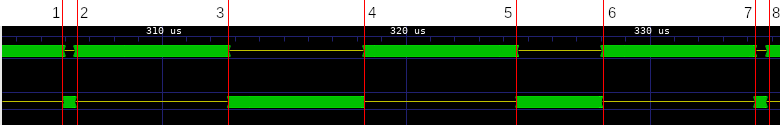
\includegraphics[width=1.\linewidth]{fb_perf}
  \caption{Performanse frame\_buffer modula}
  \label{fb_perf}
\end{figure}

Na osnovu aktivnosti donjeg interfejsa može se videti vreme rada klasifikatora, kao što se
može videti to vreme je promenljivo.
Vreme aktivnosti gornjeg interfejsa je konstantno, jer je vreme računanja
integralne slike konstantno. \\

Nakon završetka računanja integralne slike u trenutku kursora 1, klasifikator
počinje sa radom.
Rad klasifikatora traje do kursora 2.
U ovom slučaju vreme rada klasifikatora je kratko jer je prozor odbačen posle
prve etape. \\

Nakon kursora broj 2 počinje generisanje integralne slike i traje do kursora 3.
Integralna slika se generiše takođe i između kursora 4-5 i 6-7, kao što se može
videti ovo vreme je konstantno. \\

Između kursora 3-4 može se videti značajno duža aktivnost na donjem interfejsu,
posledica toga je što je klasifikator stigao do 4. etape nakon čega je odbačen prozor.
Između kursora 5-6 klasifikator odbacuje se prozor nakon 3. etape. \\

Može se videti da se u periodu između kursora 3-4 može izračunati ceo prozor integralne slike
tokom rada klasifikatora.
Kako bi se ovo odradilo potrebno je duplirati frame\_buffer memoriju.

\subsubsection{Paralelno računanje prve etape}

Kao što se vidi na grafiku(\ref{cascade_classifier_img2}) prva etapa će se
izvršiti u svakom analiziranom prozoru, procenat izvršavanja svake naredne etape
eksponencijalno opada.
Posle 5. etape procenat izvršavanja je manje od 1\%.
Prva etapa ima 9 obeležja, a zatim svaka naredna
eksponencijalno više.
Pošto će se veliki procenat vremena prilikom rada IP jezgra provesti na
računanje prve etape, računanje ove etape bi se moglo računati posebnim
prilagođenim klasifikatorom.

\subsubsection{Paralelni klasifikatori}

Kako bi se omogućio rad paralelnih klasifikatora, potrebno je izdeliti ulaznu
IMG RAM memoriju na regione.
Tako da će svaki paralelni klasifikator obrađivati svoj region. \\

U ovom slučaju treba umnožiti ii\_gen, sii\_gen, frame\_buffer, stddev module.
Adresu za čitanje koju generiše rd\_addrgen je moguće izvesti za svaki region
uvođenjem offset-a adrese, tako da rd\_addrgen nije potrebno umnožiti u ovom
slučaju.
Moguće je koristiti jednu features\_mem memoriju za sve paralelne klasifikatore,
ali u tom slučaju svi paralelni klasifikatori će raditi brzinom najsporijeg
klasifikatora.
Moguće je ponovno koristiti i memorije iz classifier modula, što uvesti isti
efekat kao i features\_mem memorije.
Aritmetičke operatore iz classifier modula je potrebno umnožiti.

\subsubsection{Računanje više obeležja u paraleli}
Kao što se može videti na blok dijagramu klasifikatora(\ref{classifier_bd})
trenutno se jedno obeležje računa u trenutku.
Potrebno je četiri takta da se površina jednog pravougaonika izračuna.
Moguće je računati 2 obeležja u paraleli.
U tom slučaju bi frame\_buffer memorija bila duplirana zbog većeg broja portova
za čitanje.
Dok bi features\_mem memorija bila značajno komplikovanija, kao i classifier modul.

\subsubsection{Računanje skaliranih slika u paraleli}

Kao što se može videti na slici(\ref{image_pyramid}) originalna slika se mora
obrađivati više puta nakon skaliranja.
Rezultati obrade slika na različitim skalama nemaju međusobnu zavisnost, zbog
toga je moguće obrađivati ih u paraleli. \\

Primenom ove optimizacije ne može se dobiti linearno uvećanje brzine.
Pošto je najviše vremena potrebno da se obradi originalna slika, dok je za svaku
narednu skaliranu sliku potrebno sve manje vremena za obradu.
Dobitak performansi ove optimizacije verovatno nije opravdan za dodatne
hardverske resurse.
